
%(BEGIN_QUESTION)
% Copyright 2012, Tony R. Kuphaldt, released under the Creative Commons Attribution License (v 1.0)
% This means you may do almost anything with this work of mine, so long as you give me proper credit

In this process, hot steam is used to ``strip'' volatile sulfur compounds from process water, inside a vessel called a {\it stripping tower}.  A flow control system (loop \#28) regulates the amount of stripping steam admitted to the tower:

$$\includegraphics[width=15.5cm]{i0007rx01.eps}$$

Suppose the last instrument technician to calibrate the steam flow transmitter (FT-28) made a mistake, and the transmitter consistently reads 1.2 pound per minute more steam flow than there actually is going through the pipe.  For example, if the actual steam flow is 6.9 pounds per minute, the transmitter outputs a current signal corresponding to 8.1 pounds per minute.

\vskip 10pt

Describe in detail the effect this mis-calibration will have on the performance of the steam flow control system.

\vskip 20pt \vbox{\hrule \hbox{\strut \vrule{} {\bf Suggestions for Socratic discussion} \vrule} \hrule}

\begin{itemize}
\item{} Perform a ``thought experiment'' where you borrow a friend's car to drive, not knowing the this car's speedometer reads faster than you are actually traveling.  What speed will you actually be driving as you attempt to obey the speed limit?
\item{} How do you suppose this miscalibration will affect the performance of the sour water stripping unit?
\item{} Would this miscalibration be evident to an operator looking at the ``faceplate'' (graphic display) of FIC-28?  Why or why not?
\item{} For those who have studied calibration errors, would you characterize this error as a {\it zero shift}, a {\it span shift}, a {\it non-linearity}, or {\it hysteresis}?
\item{} Explain why nearly every automatic control valve in this process is flanked by two ``block'' hand valves (one upstream and one downstream) and paralleled by a ``bypass'' hand valve.
\end{itemize}

\underbar{file i02928}
%(END_QUESTION)





%(BEGIN_ANSWER)


%(END_ANSWER)





%(BEGIN_NOTES)

The steam flow will end up being 1.2 lb/minute {\it less} than it should be as a result of this transmitter miscalibration.  For example, if the controller's setpoint is 5.5 lb/min and the control system is working well, the actual steam flow will settle at 4.3 lb/min.



\filbreak \vskip 20pt \vbox{\hrule \hbox{\strut \vrule{} {\bf Virtual Troubleshooting} \vrule} \hrule}

\noindent
{\bf Predicting the effect of a given fault:} present each of the following faults to the students, one at a time, having them comment on all the effects each fault would produce.

\begin{itemize}
\item{} 
\item{} 
\item{} 
\end{itemize}

\vskip 10pt


\noindent
{\bf Identifying possible/impossible faults:} present symptoms to the students and then have them determine whether or not a series of suggested faults could account for all the symptoms, explaining {\it why} or {\it why not} for each proposed fault:

\begin{itemize}
\item{} Symptom: {\it TG-344 reads excessively high in temperature}
\item{} TV-21 upstream block valve left shut -- {\bf Yes}
\item{} TV-21 downstream block valve left shut -- {\bf Yes}
\item{} TV-21 bypass valve left open -- {\bf No}
\item{} TIC-21 left in manual mode -- {\bf Yes}
\item{} TT-21 failed with high signal -- {\bf No}
\item{} TT-21 failed with low signal -- {\bf Yes}
\item{} TIR-21 chart recorder runs out of paper -- {\bf No}
\item{} Pump P-101 shut off -- {\bf Yes}
\item{} Heat exchanger E-9 upstream block valve left shut -- {\bf No}
\item{} Heat exchanger E-9 bypass valve left open -- {\bf Yes}
\end{itemize}



\vskip 10pt


\noindent
{\bf Determining the utility of given diagnostic tests:} imagine the cooling water valve TV-21 begins to badly leak by in this system (but don't tell this to students!).  Present the operator's observation(s) to the students, have them consider possible faults and diagnostic strategies, and then propose the following diagnostic tests one by one.  Have students rate the value of each test, determining whether or not each test would give us useful information (i.e. tell us something we don't already know).  Also have students describe what re

\begin{itemize}
\item{} {\it TIC-21 reads below setpoint (PV = 235 deg F ; SP = 297 deg F)}
\item{} Check TIC-21 output (should be 0\%) -- {\bf Yes}
\item{} Check TIR-21 reading -- {\bf Yes}
\item{} Check PG-441 reading -- {\bf No}
\item{} Check TG-344 reading -- {\bf Yes}
\item{} Inspect TV-21 valve stem to see what position it's in -- {\bf Yes}
\item{} Shut upstream or downstream block valve for TV-21-- {\bf Yes}
\item{} Open bypass valve around TV-21-- {\bf No}
\item{} Check indiation of FI-97 -- {\bf Yes}
\item{} Place TIC-21 in manual and open TV-21 -- {\bf No}
\end{itemize}


\vskip 10pt


\noindent
{\bf Diagnosing a fault based on given symptoms:} imagine the ??? fails ??? in this system (but don't tell this to students!).  Present the operator's observation(s) to the students, have them consider possible faults and diagnostic strategies, and then tell them the results of tests they propose based on the following symptoms, until they have properly identified the nature and location of the fault:

\begin{itemize}
\item{} 
\item{} 
\item{} 
\end{itemize}



%INDEX% Basics, control loop troubleshooting: determining effect of specified fault(s)
%INDEX% Process: sour water stripping tower (realistic P&ID shown)

%(END_NOTES)


